\documentclass[10pt]{standalone}
\usepackage{pgfplots}
\pgfplotsset{compat=1.15}
\usepackage{mathrsfs}
\usepackage{amssymb}
\usepackage{amsmath}
\usetikzlibrary{arrows}
\pagestyle{empty}

\begin{document}



\tikzset{every picture/.style={line width=0.75pt}} %set default line width to 0.75pt        

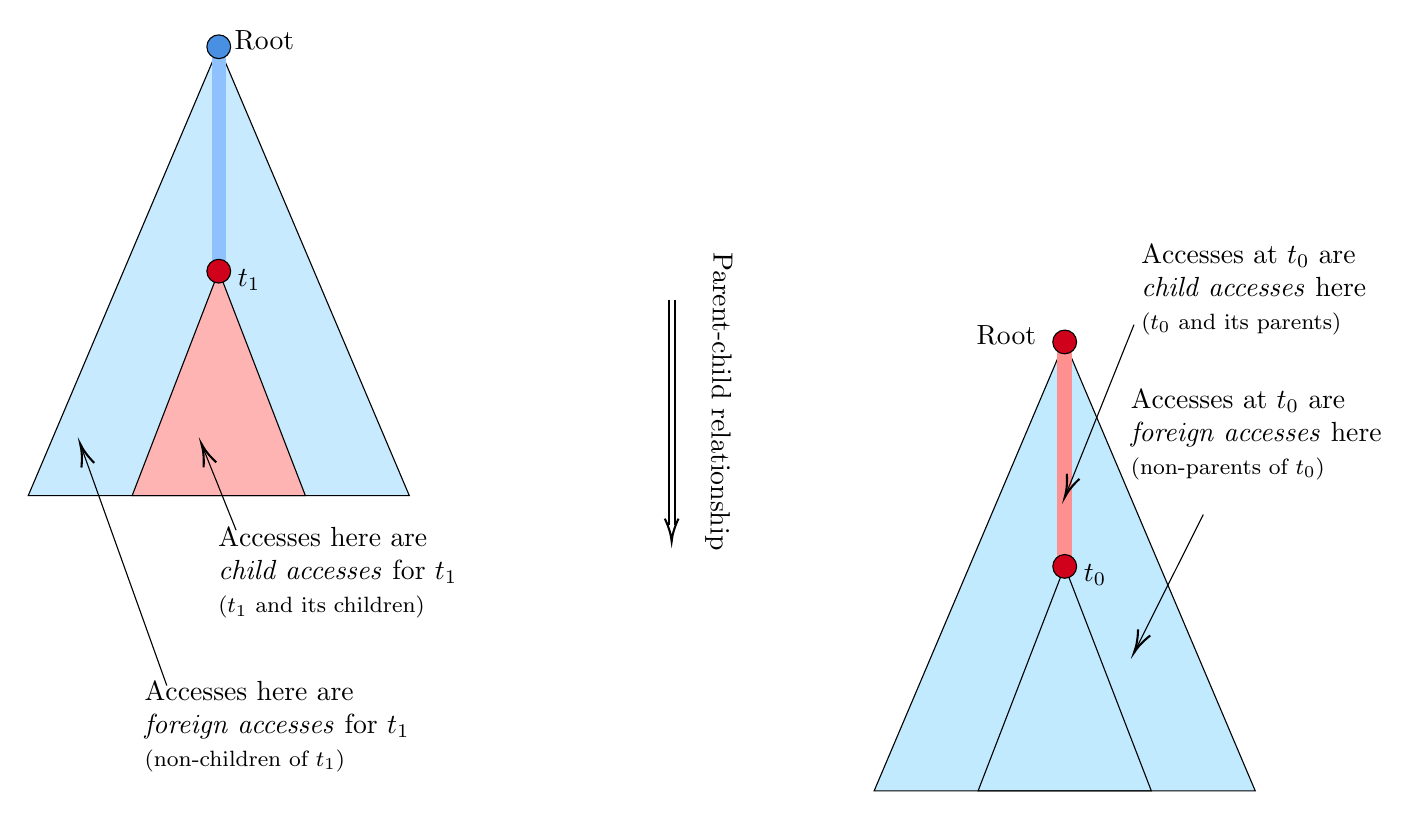
\begin{tikzpicture}[x=0.75pt,y=0.75pt,yscale=-1,xscale=1]
%uncomment if require: \path (0,467); %set diagram left start at 0, and has height of 467

%Shape: Triangle [id:dp7986839503012023] 
\draw  [fill={rgb, 255:red, 200; green, 234; blue, 255 }  ,fill opacity=1 ] (111.8,18.15) -- (203.61,234.43) -- (20,234.43) -- cycle ;
%Shape: Triangle [id:dp0354469856377696] 
\draw  [fill={rgb, 255:red, 255; green, 180; blue, 180 }  ,fill opacity=1 ] (111.8,126.29) -- (153.53,234.43) -- (70.07,234.43) -- cycle ;
%Shape: Triangle [id:dp1861807277968478] 
\draw  [color={rgb, 255:red, 0; green, 0; blue, 0 }  ,draw opacity=1 ][fill={rgb, 255:red, 194; green, 234; blue, 255 }  ,fill opacity=1 ] (519.37,160.38) -- (611.17,376.66) -- (427.56,376.66) -- cycle ;
%Shape: Triangle [id:dp38989437130052285] 
\draw   (519.37,268.52) -- (561.1,376.66) -- (477.64,376.66) -- cycle ;
%Straight Lines [id:da40615578262469076] 
\draw [line width=0.75]    (331.5,140) -- (331.5,248.46)(328.5,140) -- (328.5,248.46) ;
\draw [shift={(330,256.46)}, rotate = 270] [color={rgb, 255:red, 0; green, 0; blue, 0 }  ][line width=0.75]    (10.93,-3.29) .. controls (6.95,-1.4) and (3.31,-0.3) .. (0,0) .. controls (3.31,0.3) and (6.95,1.4) .. (10.93,3.29)   ;
%Straight Lines [id:da5527549140597704] 
\draw [color={rgb, 255:red, 255; green, 144; blue, 144 }  ,draw opacity=1 ][fill={rgb, 255:red, 255; green, 161; blue, 161 }  ,fill opacity=1 ][line width=5.25]    (519.37,160.38) -- (519.37,268.52) ;
%Shape: Ellipse [id:dp2835241193936743] 
\draw  [fill={rgb, 255:red, 208; green, 2; blue, 27 }  ,fill opacity=1 ] (513.63,268.52) .. controls (513.63,265.37) and (516.2,262.8) .. (519.37,262.8) .. controls (522.54,262.8) and (525.11,265.37) .. (525.11,268.52) .. controls (525.11,271.68) and (522.54,274.24) .. (519.37,274.24) .. controls (516.2,274.24) and (513.63,271.68) .. (513.63,268.52) -- cycle ;
%Shape: Ellipse [id:dp9384690640661182] 
\draw  [fill={rgb, 255:red, 208; green, 2; blue, 27 }  ,fill opacity=1 ] (513.63,160.38) .. controls (513.63,157.23) and (516.2,154.67) .. (519.37,154.67) .. controls (522.54,154.67) and (525.11,157.23) .. (525.11,160.38) .. controls (525.11,163.54) and (522.54,166.1) .. (519.37,166.1) .. controls (516.2,166.1) and (513.63,163.54) .. (513.63,160.38) -- cycle ;
%Straight Lines [id:da660876006399563] 
\draw    (86.77,325.93) -- (45.71,211.36) ;
\draw [shift={(45.04,209.47)}, rotate = 70.29] [color={rgb, 255:red, 0; green, 0; blue, 0 }  ][line width=0.75]    (10.93,-3.29) .. controls (6.95,-1.4) and (3.31,-0.3) .. (0,0) .. controls (3.31,0.3) and (6.95,1.4) .. (10.93,3.29)   ;
%Straight Lines [id:da8758041073375903] 
\draw    (120.15,251.07) -- (104.2,211.33) ;
\draw [shift={(103.46,209.47)}, rotate = 68.13] [color={rgb, 255:red, 0; green, 0; blue, 0 }  ][line width=0.75]    (10.93,-3.29) .. controls (6.95,-1.4) and (3.31,-0.3) .. (0,0) .. controls (3.31,0.3) and (6.95,1.4) .. (10.93,3.29)   ;
%Straight Lines [id:da3115259932914679] 
\draw    (552.75,152.07) -- (520.11,233.39) ;
\draw [shift={(519.37,235.25)}, rotate = 291.87] [color={rgb, 255:red, 0; green, 0; blue, 0 }  ][line width=0.75]    (10.93,-3.29) .. controls (6.95,-1.4) and (3.31,-0.3) .. (0,0) .. controls (3.31,0.3) and (6.95,1.4) .. (10.93,3.29)   ;
%Straight Lines [id:da9244281537647517] 
\draw    (586.13,243.57) -- (553.65,308.33) ;
\draw [shift={(552.75,310.12)}, rotate = 296.64] [color={rgb, 255:red, 0; green, 0; blue, 0 }  ][line width=0.75]    (10.93,-3.29) .. controls (6.95,-1.4) and (3.31,-0.3) .. (0,0) .. controls (3.31,0.3) and (6.95,1.4) .. (10.93,3.29)   ;
%Straight Lines [id:da730129465065093] 
\draw [color={rgb, 255:red, 144; green, 193; blue, 255 }  ,draw opacity=1 ][fill={rgb, 255:red, 255; green, 161; blue, 161 }  ,fill opacity=1 ][line width=5.25]    (111.8,18.15) -- (111.8,126.29) ;
%Shape: Ellipse [id:dp31131141671438556] 
\draw  [fill={rgb, 255:red, 74; green, 144; blue, 226 }  ,fill opacity=1 ] (106.07,18.15) .. controls (106.07,14.99) and (108.63,12.43) .. (111.8,12.43) .. controls (114.97,12.43) and (117.54,14.99) .. (117.54,18.15) .. controls (117.54,21.31) and (114.97,23.87) .. (111.8,23.87) .. controls (108.63,23.87) and (106.07,21.31) .. (106.07,18.15) -- cycle ;
%Shape: Ellipse [id:dp7033192249543065] 
\draw  [fill={rgb, 255:red, 208; green, 2; blue, 27 }  ,fill opacity=1 ] (106.07,126.29) .. controls (106.07,123.13) and (108.63,120.57) .. (111.8,120.57) .. controls (114.97,120.57) and (117.54,123.13) .. (117.54,126.29) .. controls (117.54,129.45) and (114.97,132.01) .. (111.8,132.01) .. controls (108.63,132.01) and (106.07,129.45) .. (106.07,126.29) -- cycle ;

% Text Node
\draw (360.74,115.99) node [anchor=north west][inner sep=0.75pt]  [rotate=-90.61] [align=left] {Parent-child relationship};
% Text Node
\draw (119.74,124.26) node [anchor=north west][inner sep=0.75pt]    {$t_{1}$};
% Text Node
\draw (527.31,266.49) node [anchor=north west][inner sep=0.75pt]    {$t_{0}$};
% Text Node
\draw (110.32,248.43) node [anchor=north west][inner sep=0.75pt]   [align=left] {Accesses here are\\\textit{child accesses} for $\displaystyle t_{1}$\\{\footnotesize ($\displaystyle t_{1}$ and its children)}};
% Text Node
\draw (74.86,322.47) node [anchor=north west][inner sep=0.75pt]   [align=left] {Accesses here are\\\textit{foreign accesses} for $\displaystyle t_{1}$\\{\footnotesize (non-children of $\displaystyle t_{1}$)}};
% Text Node
\draw (118.17,9.23) node [anchor=north west][inner sep=0.75pt]   [align=left] {Root};
% Text Node
\draw (475.66,151.47) node [anchor=north west][inner sep=0.75pt]   [align=left] {Root};
% Text Node
\draw (555,112) node [anchor=north west][inner sep=0.75pt]   [align=left] {Accesses at $\displaystyle t_{0}$ are\\\textit{child accesses} here\\{\footnotesize ($\displaystyle t_{0}$ and its parents)}};
% Text Node
\draw (550,182) node [anchor=north west][inner sep=0.75pt]   [align=left] {Accesses at $\displaystyle t_{0}$ are\\\textit{foreign accesses} here\\{\footnotesize (non-parents of $\displaystyle t_{0}$)}};


\end{tikzpicture}

\end{document}
